\begin{figure}{!h}
	\centering
	\begin{subfigure}{0.8\linewidth}
		\centering
		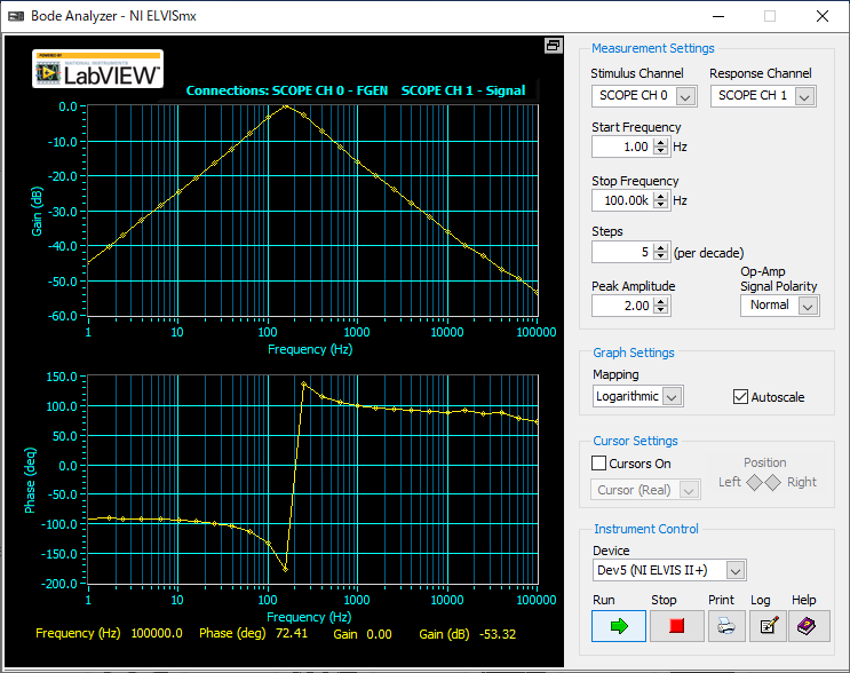
\includegraphics[width=0.8\linewidth]{src/figures/exp10/10k-low-bode.png}
		\subcaption{$R_1=\SI{10}{k\ohm}$のローパスフィルタのボード線図}\label{fig:exp10-10k-low-bode}
	\end{subfigure}
	\begin{subfigure}{0.8\linewidth}
		\centering
		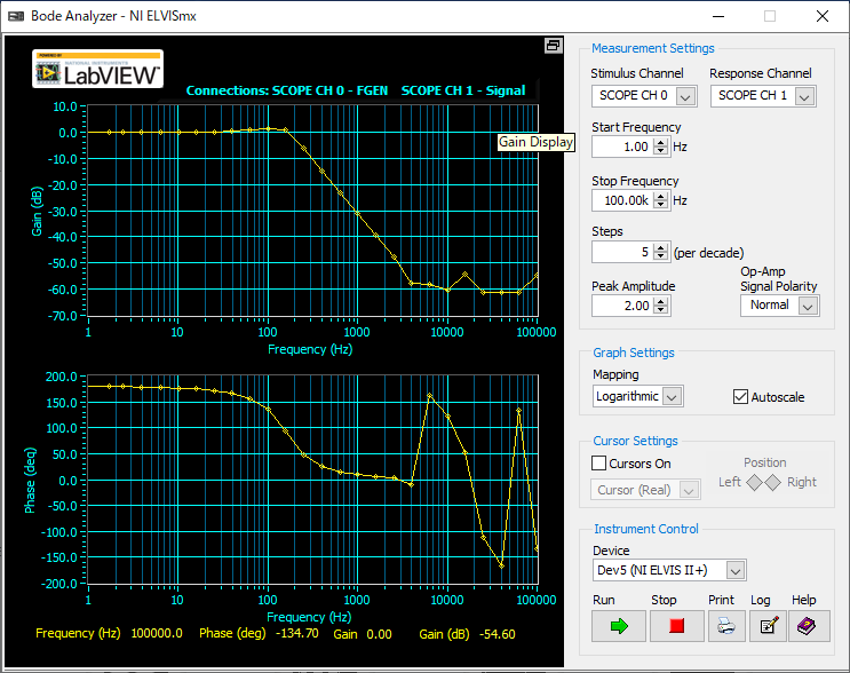
\includegraphics[width=0.8\linewidth]{src/figures/exp10/10k-band-bode.png}
		\subcaption{$R_1=\SI{10}{k\ohm}$のバンドパスフィルタのボード線図}\label{fig:exp10-10k-band-bode}
	\end{subfigure}
\end{figure}
\begin{figure}
	\centering
	\begin{subfigure}{0.8\linewidth}
		\addtocounter{subfigure}{2}
		\centering
		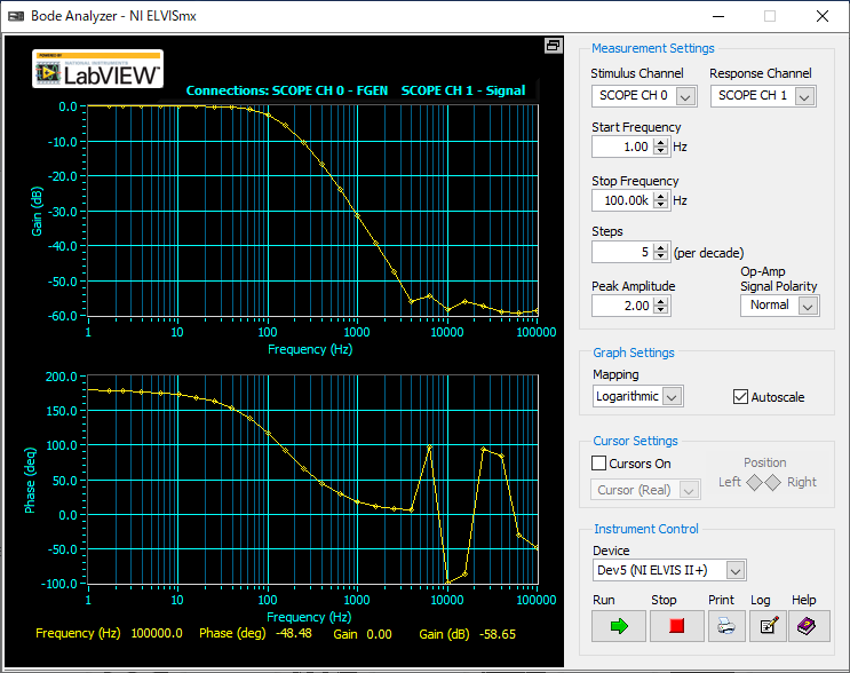
\includegraphics[width=0.8\linewidth]{src/figures/exp10/5k-band-bode.png}
		\subcaption{$R_1=\SI{5}{k\ohm}$のバンドパスフィルタのボード線図}\label{fig:exp10-5k-band-bode}
	\end{subfigure}
	\begin{subfigure}{0.8\linewidth}
		\centering
		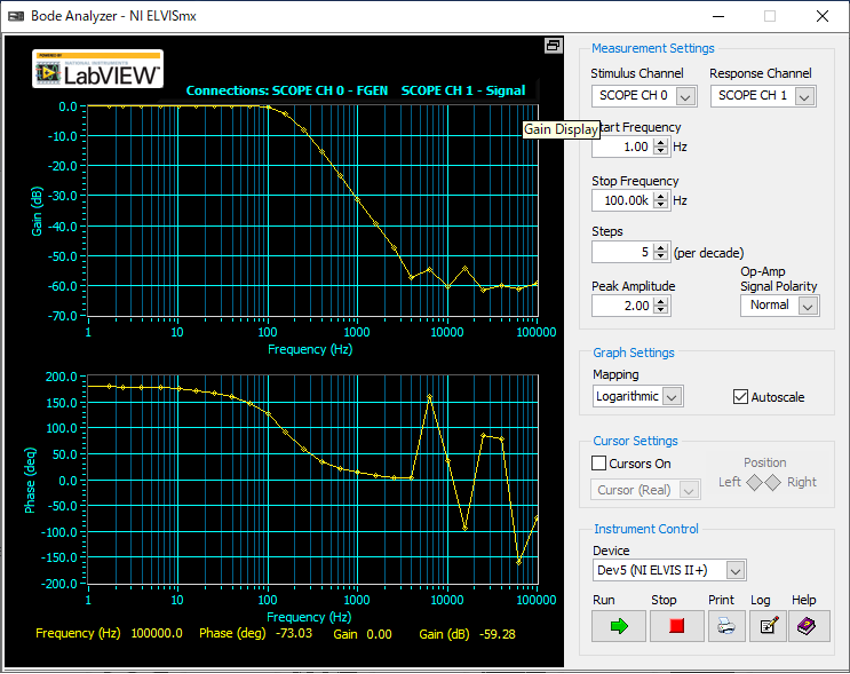
\includegraphics[width=0.8\linewidth]{src/figures/exp10/7k-band-bode.png}
		\subcaption{$R_1=\SI{7}{k\ohm}$のバンドパスフィルタのボード線図}\label{fig:exp10-7k-band-bode}
	\end{subfigure}
\end{figure}
\begin{figure}
	\centering
	\begin{subfigure}{0.8\linewidth}
		\addtocounter{subfigure}{4}
		\centering
		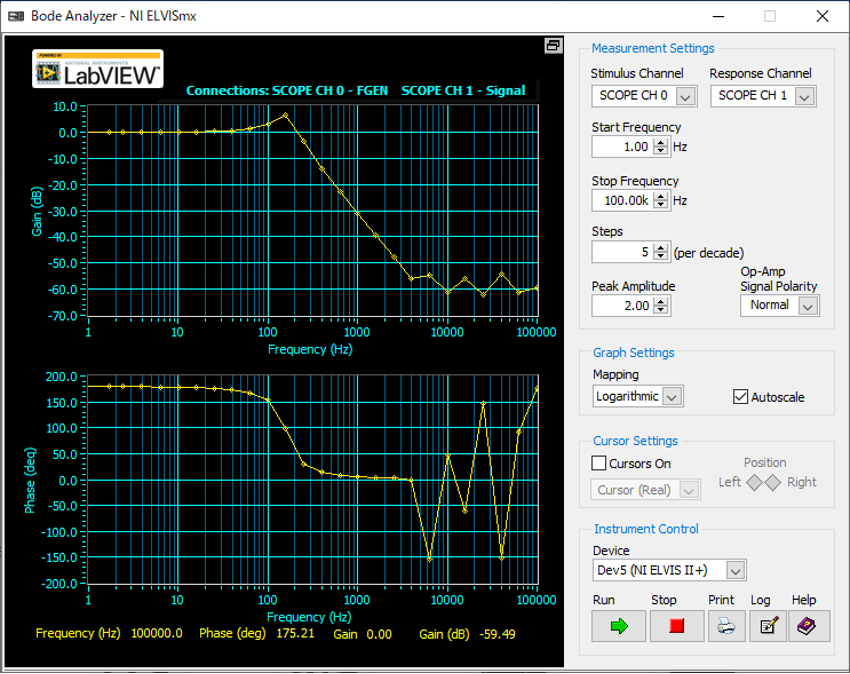
\includegraphics[width=0.8\linewidth]{src/figures/exp10/20k-band-bode.png}
		\subcaption{$R_1=\SI{20}{k\ohm}$のバンドパスフィルタのボード線図}\label{fig:exp10-20k-band-bode}
	\end{subfigure}
	\caption{実験10で作成したバイカット型フィルタのボード線図}\label{fig:exp10-bode}
\end{figure}
